\chapter{Model architecture}\label{chap:architecture}
For our end-to-end SVG generation method, we build upon the work of Sketch-RNN~\citeauthor{ha2017neural} and use a similar bidirectional sequence-to-sequence variational autoencoder model~\cite{ha2017neural}.
We maintain a similar encoder and latent space architecture, but we modify the decoder to output parameters corresponding to four probability distributions instead of two.
In Sketch-RNN, the decoder output parameterizes a Gaussian Mixture Model (GMM) for the pen coordinates as well as a categorical distribution for the pen state (\textit{pen up}, \textit{pen down}, or \textit{end drawing}).
To model general SVG commands, we modify the decoder to output parameters for three GMMs, one for each of the possible control points in a cubic B\'ezier curve (except the start position, since we assume we start drawing from the pen's current location), as well as for a categorical pen state distribution.
An overview of the model architecture is depicted in Figure~\ref{fig:architecture}.

\section{VAE modules}
Dual RNNs are used in the encoder module, one for modeling forward and one for modeling backward sequences of feature vectors, with each feature vector representing a single SVG command.
Both RNNs use LSTM cells with layer normalization, as introduced in~\cite{ba2016layer}.
After transforming an input SVG into a sequence of feature vectors $S = (S_1, S_2, \cdots, S_n)$ which includes padding with \textit{end drawing} vectors to ensure $S$ is length $n_\text{max}$, each $S_i$ is passed in to the encoder RNNs in the appropriate order.
The final hidden states of both RNNs, $h_\leftarrow$ from the backward encoder and $h_\to$ from the forward encoder, are concatenated to form a combined output $h$.
Assuming the latent space vector has dimension $n_z$, this output is then transformed into $\mu$ and $\sigma$ vectors using a fully connected layer (and an exponentiation operation to produce a non-negative $\sigma$) such that both vectors have dimension $n_z$.

\begin{figure}[h]
\centering
\caption[An overview of the basic SVG model architecture]{An overview of the basic SVG model architecture.
Although similar overall to~\cite{ha2017neural}, the model is adapted such that $y_i$ parameterizes three location GMMs and a pen state distribution.\label{fig:architecture}}
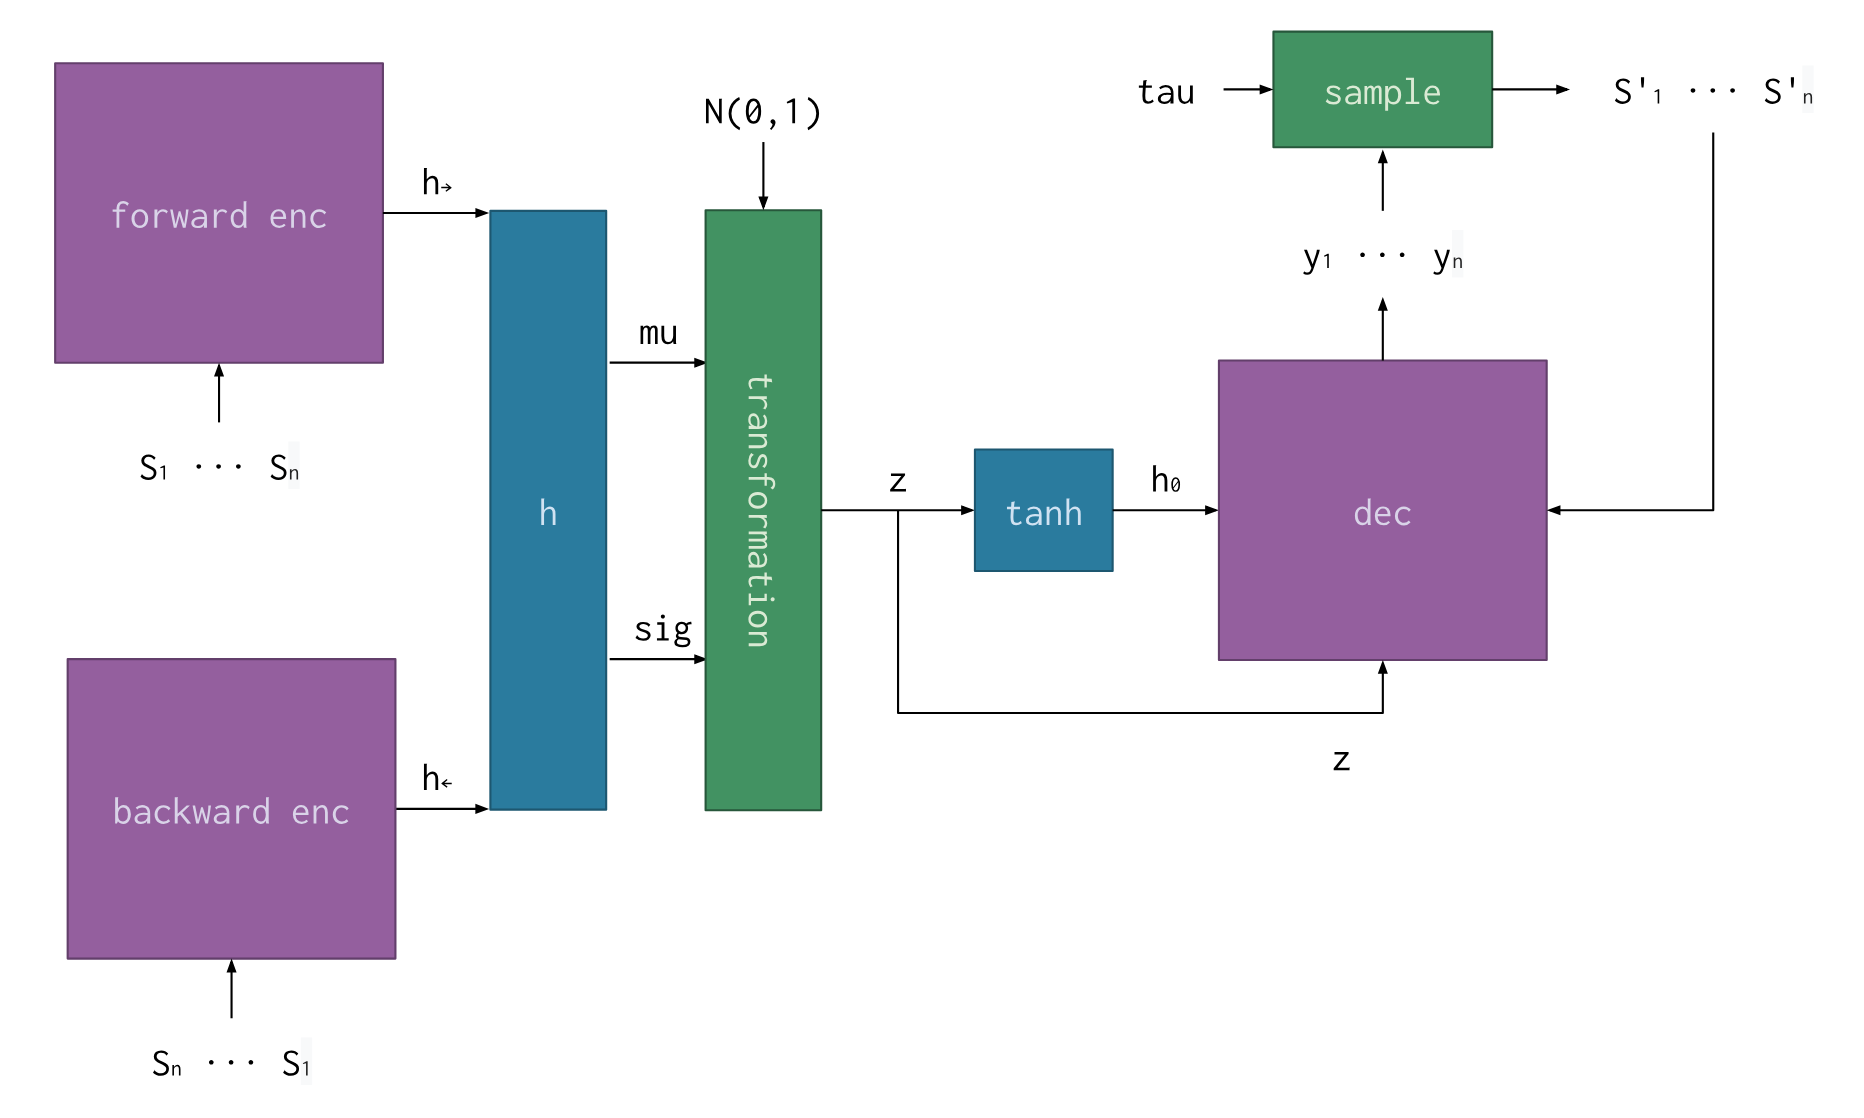
\includegraphics[width=\textwidth]{figures/architecture}
\end{figure}

The resulting $\mu$ and $\sigma$ vectors are combined with a vector $\mathcal{N}$ of $n_z$ normally distributed Gaussian samples from $\mathcal{N}(0,1)$ to create a random latent vector $z$, with $z = \mu + \sigma \circ \mathcal{N}$.

A single-layer network takes in $z$ and outputs the initial input $h_0$ to the decoder module.
Each cell in the decoder takes in $z$, the output from the previous cell $h_i$, and the generated output SVG command $S'_i$.
The output from a decoder cell $y_i$ is a vector composed of three values for the categorical pen state distribution plus parameters for each of the three location GMM models.

The number of normal distributions in each location GMM is a tunable hyperparameter.
By default, each GMM contains 20 normal distributions, and each distribution is parameterized by means and standard deviations for both the $x$ and $y$ locations and a correlation between $x$ and $y$ ($\mu_x$, $\sigma_x$, $\mu_y$, $\sigma_y$, $\rho_{xy}$).
The models in the GMM also each have a mixture weight $\pi$.
The values corresponding to $\sigma$ values in $y_i$ are again exponentiated to produce non-negative standard deviations, and we apply $\tanh$ operations to the values corresponding to $\rho$ values to ensure they produce correlations between -1 and 1. 

To generate $S_i$, each GMM is sampled to produce pen locations $x$ and $y$ for each coordinate in the SVG feature vector, and the pen state distribution is sampled to generate one of $\{p_d, p_u, p_e\}$, corresponding to \textit{pen down}, \textit{pen up}, and \textit{end drawing}.
A temperature multiplier ($\tau$) is also used when sampling from GMMs and from the pen state distribution to adjust the randomness of the output, allowing for control over how expected (and thus how similar to existing inputs) the output is.
Finally, all generated $S_i$ are ordered in sequence to produce a generated list of SVG commands. The specific transformation from the three coordinates in the feature vector to the output SVG command parameters varies (see Chapter~\ref{chap:feature-variation}), but all feature encodings we use require three coordinates. 

The model is also capable of generating unconditional output, in which no input SVG is supplied.
The produced result is an unseen example not explicitly related to any particular image in the dataset.
We train the model to produce unconditional output by setting the decoder's initial states to 0 and treating it as a standalone RNN without a $z$ input.
